\documentclass[letterpaper, 12pt]{report}
\usepackage[utf8]{inputenc}
\usepackage[spanish]{babel}
\usepackage{cite,url,graphicx,amsmath,enumitem}
\usepackage{fullpage}
\usepackage{authblk}

%para definir bibliografia en referencias
%\usepackage{etoolbox}
%\makeatletter
%\patchcmd{\thebibliography}{%
%  \chapter*{\bibname}\@mkboth{\MakeUppercase\bibname}{\MakeUppercase\bibname}}{%
%  \chapter*{Bibliografía}}{}{}
%\makeatother

\title{Estudio de algoritmos de calendarización para flujos de trabajo}
\author{Fernando Aguilar Reyes}

\affil{Tesina para obtener el título de Ingeniero en Computación \\
       Instituto Tecnológico Autónomo de México \\
     Río Hondo \#1, Progreso Tizapán, Del. Álvaro Obregón, 01080 \\
     México, Distrito Federal \\}


%interlineado
\renewcommand{\baselinestretch}{1.5}

\begin{document}

\maketitle

\tableofcontents

\listoffigures

\chapter{Introducción}
Cada día, los cómputos son más complejos. Hay bancos que procesan millones de transacciones diarias. Las películas de animación requieren vastos tiempos de cómputo. Muchos proyectos de computación científica requieren hacer numerosos cálculos para llegar a resultados pertinentes. ¿Qué tienen en común todas estas aplicaciones? Ya hemos mencionado que toman mucho tiempo calcularse. Entonces, es natural pensar que se puede distribuir el gran trabajo que requieren estos proyectos entre varias computadoras para disminuir el tiempo total de ejecución y de esta forma, tener una solución escalable. 

Lograr esta paralelización requiere un esfuerzo por parte del desarrollador de la solución. Aunque estas técnicas de paralelización son muy efectivas, éstas son aplicadas cuando el problema a resolver ha sido bien definido y cuando sólo hay una instancia del problema. Ahora bien, cuando la solución involucra varios pasos que están relacionados entre sí, por ejemplo, que el programa C requiera de la salida del programa A y del programa B para que pueda funcionar. O, cuando estamos definiendo los grandes bloques de solución del problema, hay una cierta secuencia que debemos seguir y, dentro de dicha secuencia, hay algunos pasos que podemos resolver de manera concurrente. Por lo tanto, estamos haciendo un \emph{modelo} de nuestro problema.

Este modelo también es llamado \emph{flujo de trabajo}. De manera muy abstracta, un modelo de trabajo es un conjunto de pasos que modelan la ejecución de un proceso. Este concepto ha sido aplicado en numerosas áreas. En el ámbito de los negocios, se utiliza diagramas dibujados con los bloques y reglas del \emph{Bussiness Process Execution Language} para modelar procesos de negocio.

En el ámbito de las ciencias en computación, los flujos de trabajo son aplicados para modelar problemas que requieran varios pasos para su solución. Algunos flujos de trabajo requieren mucho tiempo tiempo de ejecución para sus pasos, como son el caso de los flujos de trabajo científicos. Otros flujos de trabajo son muy simples pero  se requieren que se ejecuten muchos de éstos. De esta forma, es desable distribuir la ejecución de éstos flujos de trabajo entre varias computadoras. Si bien es posible paralelizar algunos pasos de la ejecución de nuestro flujo de trabajo utilizando las técnicas antes mencionadas, hay restricciones de orden que se deben respetar, por lo cual, se debe planear la ejecución del flujo de trabajo.

Hay varias maneras de hacer esta planeación de la ejecución, también llamada \emph{calendarización}. Cabe aclarar que definimos la calendarización como la asignación de recursos a tareas de tal modo que se ejecuten todas las tareas. Con ello, se desea encontrar una forma óptima de hacer esta calendarización, como reducir el tiempo de ejecución total del flujo de trabajo. Sin embargo, con la aparición del cómputo en la nube, es posible ejecutar nuestro flujo de trabajo con otras restricciones, como minimizar el presupuesto necesario para la ejecución del flujo afectando el tiempo de ejecución.

%mencionar instruction level paralelism, task level paralelism, 

%uml, bepl para software y negocios, buscar los que vienen en el paper de hierarchical scheduling for swindew-c

En esta tesina se hace un estudio de los principales algoritmos de calendarización de flujos de trabajo, con énfasis en los algoritimos utilizados en cómputo distribuido, en especial en cómputo en la nube. En el capítulo 2 se habla de un estudio detallado del concepto de flujos de trabajo y su aplicación en computación. El capítulo 3 trata los principales enfoques de cómputo distribuido para ejecutar estos flujos. En el capítulo 4 se hace un estudio de los principales algoritmos de calendarización de los flujos. Finalmente, en el capítulo 6 discutiremos algunas conclusiones sobre el análisis de estos algoritmos.


\chapter{Flujos de trabajo}

\section{Definición y ejemplos}
Un flujo de trabajo es un conjunto de pasos que modelan la ejecución de un proceso \cite{gutierrez2012agent}. En la literatura especializada, los flujos de trabajos también son conocidos como \emph{workflows}. En particular, se estudian a los flujos de trabajo utilizados para vislumbrar la ejecución de un proceso de cómputo. A continuación, se muestran algunos ejemplos de estos flujos de trabajo.

\subsection{Anotación de proteínas}
En el proyecto \emph{e-Protein}, realizado por la Escuela Imperial de Londres, se realizó un flujo de trabajo para la anotación de proteínas. El objetivo del proyecto \cite{o2004mapping} era la identificación y anotación de partes de proteínas que expliquen su estructura y su función. En la figura \ref{fig:iceni-workflow} se muestra el flujo de trabajo desarrollado, donde las cajas representan los programas que son ejecutados para cada paso del proceso de anotación, y las líneas que conectan a las cajas representan las dependencias de datos entre los programas, es decir, si una caja tiene una línea que apunta a ella, significa que dicho programa depende de otro porgrama determinado por el otro extremo de la flecha.

\begin{figure}
    \begin{center}
        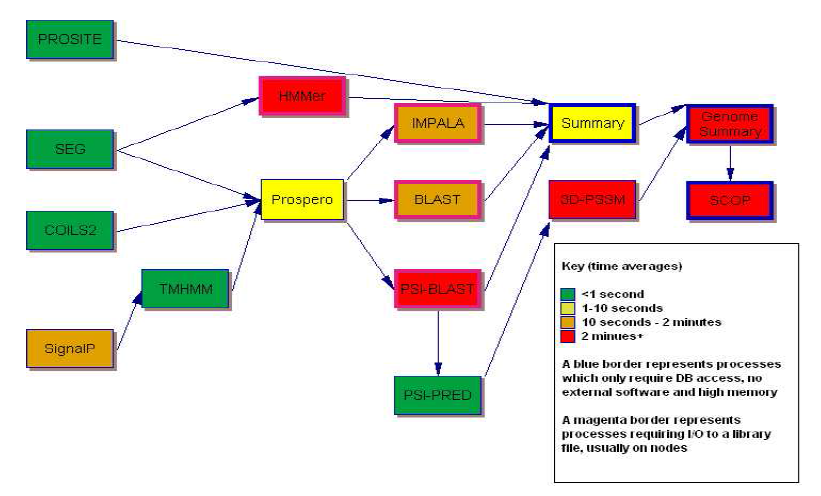
\includegraphics[width=0.8\textwidth]{imagenes/iceni-workflow}
    \end{center}
    \caption{Flujo de trabajo para la anotación de proteínas, diseñado en la Escuela Imperial de Londres para el proyecto \emph{e-Protein}.}
    \label{fig:iceni-workflow}
\end{figure}


\subsection{Curvas de amenaza sísmica}
Otro notable ejemplo es el proceso para generar curvas de amenaza que describen las probabilidades de que ocurra un temblor en una determinada área. Para elaborar estas curvas, los científicos del Centro de Terremotos del Sureste de California (SCEC por sus siglas en inglés) tienen que realizar una gran cantidad de simulaciones para que sus resultados puedan ser combinados y expresados en la curva de amenaza \cite{deelman2006managing}. El flujo de trabajo para generar la curva de amenaza se muestra en la figura \ref{fig:scec-workflow}.

\begin{figure}
    \begin{center}
        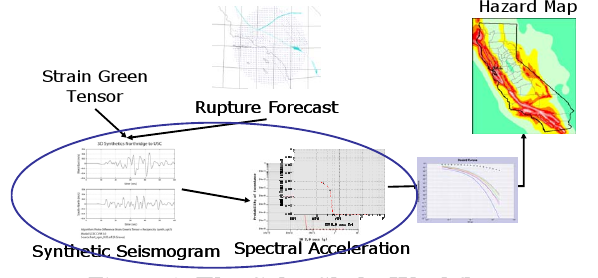
\includegraphics[width=0.8\textwidth]{imagenes/scec-workflow}
    \end{center}
    \caption{Flujo de trabajo para generar curvas de amenaza, elaborado por el SCEC.}
    \label{fig:scec-workflow}
\end{figure}

\section{Estructura de los flujos de trabajo}
Como hemos visto en los dos ejemplos anteriores, los flujos de trabajo presentados describen los \emph{pasos} que necesitan para calcular la solución de un problema. En éstos, no se ha hablado sobre detalles para hacer los cómputos necesarios para cada flujo. Tampoco definen las plataformas de cómputo en que se ejecutan estos flujos. Tan sólo definen los grandes pasos para solucionar el problema y las dependencias que tienen estos pasos. 

Ahora, es muy común que estas dependencias estén dictadas por los datos que requiere cada paso para funcionar. Sin embargo, hay situaciones en los que los pasos del flujo no requieren los datos del paso anterior para funcionar, sino que las dependencias están marcadas por el orden temporal que deben seguir estos pasos. Así, se puede notar una ambigüedad en la definición de un flujo de trabajo.

\subsection{Perspectivas de los flujos de trabajo}
El trabajo de Van der Aalst et al. \cite{van2003workflow} identifica una serie de perspectivas vislumbrados en las definiciones de las especificaciones de un flujo de trabajo en las que se basan los sistemas que administran la ejecución de éstos. Las cuatro perspectivas se enuncian a continuación:
%En esta tesis, tomaremos estas perspectivas a manera de una clasificación de flujos de trabajo basadas en la forma en que describen sus dependencias

\begin{itemize}

\item{\textbf{Perspectiva de control de flujo.} Describe las relaciones de las actividades (pasos) con estructuras de control, tales como: secuencia, decisión, ejecución de actividades en paralelo y punto de sincronización conjunta\footnote{Esta estructura de control también es conocida como \emph{join synchronization}}.}

\item{\textbf{Perspectiva de datos.} En ella, los flujos de trabajo describen las entradas y salidas de datos, tanto de ejecución como de control, que se tienen en cada actividad del flujo. También se toma en cuenta los datos locales a cada actividad; es decir, que sólo son necesarios dentro del contexto de ésta.}

\item{\textbf{Perspectiva de recursos.} Muestra cuáles son los recursos con los que se cuentan para ejecutar el flujo de trabajo y la forma en que estos recursos se encuentran organizados. Estos recursos pueden ser desde entidades de cómputo hasta roles con responsabilidades específicas cumplidas por actores humanos.}

\item{\textbf{Perspectiva operacional.} Aquí se detallan las operaciones elementales necesarias en cada actividad para ejecutar el flujo de trabajo. Estos detalles incluyen las transferencias de datos entre las operaciones y su correspondencia en programas.}

\end{itemize}

Cabe aclarar que estas perspectivas están relacionadas entre sí de modo que el control de flujo es la base en la que descansan las demás perspectivas. Esto es porque la perspectiva de datos requiere que el control de flujo tenga los datos de entrada y salida como prueba de que se cumplieron las pre y post-condiciones de cada actividad, respectivamente; la perspectiva de recursos define con qué se ejecutarán y almacenará los datos del flujo de trabajo; mientras que la perspectiva operacional trata los detalles sobre cómo se utilizan \emph{físicamente} los recursos, los datos y los programas a lo largo del flujo de trabajo.

\section{Calendarización como control de flujo}

El hecho de que la perspectiva de control de flujo sea la base de las demás perspectivas indica que la forma en que controla la ejecución del flujo determina de manera fundamental el rendimiento de la ejecución total de una instancia del flujo. Por lo tanto, es de vital importancia encontrar métodos de calendarización que permitan encontrar correspondencias entre recursos y actividades que cumplan con los requisitos dictados en las especificaciones examinadas en la perspectiva del control del flujo y que también maximicen el rendimiento de la ejecución de todo el flujo en general.

En este trabajo, se establecerán las siguientes consideraciones para limitar el estudio de los algoritmos de calendarización, a saber:

\begin{itemize}
\item{Los flujos de trabajo están representados como \emph{grafos dirigidos acíclicos}, con el objetivo de simplificar el estudio}

\item{Las tareas (o actividades) de los flujos de trabajo son consideradas \emph{atómicas}, i.e., una tarea no puede ejecutarse incompletamente. Algunos sistemas de administración de ejecución de flujos de trabajo tienen mecanismos para lidiar con estos errores, pero el estudio de éstos queda fuera de los límites de este trabajo.}

\item{La información de las \emph{demás perspectivas} se puede requerida, dependiendo si el mecanismo de calendarización lo considere necesario para tomar mejores decisiones.}
\end{itemize}

%conclusiones:
% - representar como DAG's porque es sencillo y expresivo (balanceado)
% - tareas atómicas
% - la información de las demás perspectivas se puede requerir o no, dependiendo de como lo requiera el calendarizador.


%ejemplo: ICENI tiene partes paralelas, que no requieren de ciertos datos para operar
%ejemplo: Si hablas de orden,
%poner ejemplos donse se ejemplifique esta calendarización

%clasificados de acuerdo a dependencias (de orden, o de datos)


%clasificados de acuerdo a nivel de detalle (específico para cada plataforma)

%clasificados de acuerdo a instancias
% - pocas instancias, mucho tiempo de cómputo:
% - intensivos en instancias, pero cortos en ejecución:

%todos se pueden representar como Grafos Dirigidos Acíclicos


\chapter{Cómputo distribuido}
Los flujos de trabajo requieren de recursos de cómputo para su ejecución. En los ejemplos anteriores se mencionaron aplicaciones científicas que, por su naturaleza, requieren vasto tiempo de ejecución para llevarse a cabo. Por otro lado, también existen aplicaciones de negocio que, si bien son computacionalmente sencillas, se requiere ejecutar una gran cantidad de instancias de estos flujos de trabajo. Por ello, ejecutar cualquiera de estos flujos de trabajo en una sola computadora resulta prohibitivo. Así, se hace uso de varias computadoras para distribuir el esfuerzo para correr estos grandes procesos.

Dependiendo de cómo estén organizados estas computadoras, se definen los enfoques para correr los flujos de trabajo con cómputo distribuido.

\section{Clasificación de cómputo distribuido para la ejecución de flujos de trabajo}
Diversos enfoques se han aplicado para distribuir la ejecución de un flujo de trabajo entre varias computadoras.  De acuerdo a Buyya et al., los enfoques de cómputo más importantes para los flujos de trabajo son los \emph{clusters}, los \emph{grids} y las \emph{nubes} \cite{buyya2009cloud}. A continuación, explicaremos cada uno de los enfoques.

\subsection{Clusters}
Los \emph{clusters} son sistemas distribuidos, paralelos, compuestos de varias computadoras que son vistas como un único recurso de cómputo \cite{buyya2009cloud}. 

Un ejemplo de un cluster es la instalación de la Universidad Autónoma Metropolitana, campus Iztapalapa, llamada \emph{Aitzaloa}, compuesta por 270 nodos de cómputo, cada uno equipado con dos procesadores Intel Xeon Quad-Core y 16GB en RAM; los nodos están conectados entre sí por medio de switches Ethernet e Infiniband. La capacidad real de cómputo del cluster Aitzaloa es de 18.4 teraFLOPS \cite{uamz2013tizaloa}.

\subsection{Grids}
Los \emph{grids} son sistemas distribuidos, paralelos, compuestos de computadoras autónomas y geográficamente distribuidas que pueden trabajar en conjunto o de manera independiente de acuerdo a los objetivos, políticas y mecanismos de uno o varios administradores del sistema, es decir, un grid puede ser compartido entre varias instituciones \cite{buyya2009cloud}. 

El proyecto \emph{LANCAD}\footnote{Laboratorio Nacional de Cómputo de Alto Rendimiento} es un buen ejemplo, pues une el cluster \emph{Aitzaloa} de la UAM, el cluster de la UNAM \emph{KamBalam}, y el cluster \emph{Xiuhcoatl} del CINVESTAV por medio de una red de fibra óptica instalada en las estaciones del Sistema de Transporte Colectivo Metro. La suma de la potencias reales de cada \emph{nodo robusto} del grid es de 48.55 teraFLOPS \cite{lancad2013xiuhcoatl}.

\subsection{Nubes}
Las \emph{nubes} (clouds) son sistemas distribuidos, paralelos, compuestos de computadoras o máquinas virtuales interconectadas que son aprovisionadas para usarse como uno o varios recursos de cómputo, de acuerdo a un contrato de nivel de servicio acordado entre el proveedor de la nube y el cliente \cite{buyya2009cloud}. 

Empresas nuevas y existences proveen servicios de cómputo en la nube, tales como GoGrid, Rackspace, Amazon, Microsoft, IBM, Oracle, entre otras. La forma en que operan es la siguiente: se paga cierta cantidad por utilizar servicios de cómputo o almacenamiento durante determinado tiempo. Así, los clientes no tienen que invertir grandes cantidades de dinero para contar con una gran infraestructura como en el caso de los los clusters y los grids.



\chapter{Calendarización}


\section{Definición del problema}

\section{La complejidad de calendarizar}

\chapter{Algoritmos de calendarización}

\section{Algoritmos de Mejor Esfuerzo}

\section{Algoritmos de Calidad en el Servicio}

\chapter{Software para la administración y ejecución de flujos de trabajo}

\section{Software orientado a clusters}

\subsection{Open Grid Scheduler}

\section{Software orientado a grids}


\subsection{SwinDew-G}

\subsection{Pegasus}

\section{Software orientado a nubes}

\subsection{ANEKA}

\subsection{SwinDew-C}



\chapter{Conclusiones}

%%\renewcommand*{\bibname}{\chapter*{Referencias}}
\bibliographystyle{plain}
\bibliography{propuesta}

\end{document}